\documentclass[11pt]{article}
\usepackage{amsmath}
\usepackage{amsthm}
\usepackage{graphicx}
\usepackage{color}
\usepackage[labelsep=quad,indention=10pt]{caption}
\usepackage[labelfont=bf,list=true]{subcaption}
\usepackage[margin=1in]{geometry}

\newcommand{\executeiffilenewer}[3]{%
 \ifnum\pdfstrcmp{\pdffilemoddate{#1}}%
 {\pdffilemoddate{#2}}>0%
 {\immediate\write18{#3}}\fi%
}
\newcommand{\includesvg}[1]{%
 \executeiffilenewer{#1.svg}{#1.pdf}%
 {inkscape -z -D --file=#1.svg %
 --export-pdf=#1.pdf --export-latex}%
 \input{#1.pdf_tex}%
}

\begin{document}

\title{Array scheduling problem and array configuration schedule problem notes}
\author{Jorge Avarias \\
National Radio Astronomy Observatory\\
\texttt{javarias[at]nrao.edu}}
\maketitle

\begin{abstract}
This document introduces notes related to the observatories scheduling problem, specifically the problem is treated for radio astronomical facilities where scientific and engineering topics are covered. In particular the Atacama Large Millimiter/Submillimiter Array details are covered explaining roughly the importance of them for this new kind scheduling problem. The document tries to compare the observatory scheduling problem with classic scheduling problems, as well it tries to expose the differences among scheduling classic problems covering the current and latest studies. 
\end{abstract}

\section{Introduction}
The scheduling of proposals for astronomical observations is a complex problem, which is being treated in various ways since several decades. Although most of the modern professional observatories use certain degree of scheduling automation, there is still a huge part of human intervention to build up the daily plan, and to take last minute decisions, due to atmospheric conditions, technical failures, etc. These external parameters can vary at any time during observations, and therefore a dynamic re-scheduling is needed. In this case, external parameters can cause priority changes, as some observations may not be suitable anymore to execute under new conditions.

Usually this problem has been seen as a particular problem derived from the classic job-shop scheduling problem, which has been studied since the '60s. This approach could be useful if the astronomical facility is not based on interferometry where the quality of science value of an observation could vary greatly if the external and dynamic conditions vary. 

This document tries to give a new approach to the observatory scheduling problem covering in section \ref{sec:state-of-art} an overview of the past and current techniques used to treat the problem. A particular use of this problem problem is treated as part of the Atacama Large Millimeter/Submillimeter Array (ALMA), which currently is the largest radio interferometer telescope built in Earth. Section \ref{sec:problem} gives an overview of the general observatory scheduling problem for an radio interferometer telescope covering scientific topics, again ALMA is explained in detail.

\newpage
\section{State of the art}
\label{sec:state-of-art}

The scheduling problem is an optimization problem in which ideal jobs, also called tasks, are assigned to resources at particular times to execute these jobs, the execution of the jobs must satisfy all the constraints, this should be done in a way that the resulting schedule, the solution, is the best possible.

The most well known problem is the \textit{job-shop} scheduling problem presented by first time in 1966 by Graham \cite{graham66}. In this problem $n$ jobs of different sizes are scheduled to $m$ identical machines, where it is trying to minimize the makespan (the time taken to process all the jobs). In the definition of this problem is possible to appreciate the static nature, however     nowadays the problem can be treated as an online problem using dynamic scheduling.

The job-shop dynamic scheduling problem has been researched in the recent years, this problem adds new challenges to the online schedule, e.g. adding new jobs during the jobs execution and adding new restrictions. A simple example of dynamic schedule is found in 

\textit{(Write more about job-shop problem details)}

\subsection{Fair scheduling: Processor sharing approach}

Another approach to scheduling problem is the proportional fair scheduling studied at level of processor sharing, this problem is very common in computer science and developing of Operating System's kernels~\cite{li09} including real-time systems and in the past, in the 90's was studied in network sharing~\cite{parekh93}. 

In this problem fairness is an essential requirement of the scheduler designed for the operating system. The conventional approach is to assign to each task a weight and the scheduler ensures that each task receive time proportional to his weight~\cite{parekh93}. Since perfect fairness requires infinitesimal small scheduling quanta, which is unfeasible, all practical schedulers approximate it with the goal of obtaining small error bounds.

Most of the modern operating system have been adopted an imprecise notion of fairness that seeks prevention of the starvation and be ``reasonable'' fair at the same time~\cite{li09}. In these designs the scheduler dispatches threads in the order of threat priorities. For each thread, it assigns the threads a time slice that determines how long the thread can run once the thread dispatched. A higher priority thread receives a larger time slice, how much larger is often determined empirically, not a proportional function of the thread's priority. To facilitate fairness the scheduler also dynamically adjusts priorities, allowing the priority of a thread to decay over time or boosting it if the thread have not run for a while. Similar to time slices, the parameters of these adjustments are determined empirically using heuristic methods.  

\subsubsection{Fair scheduling theory}
Generalized Processor Sharing (GPS) is an idealized scheduling algorithm that achieves perfect fairness. All practical schedulers approximate GPS and use it as reference to measure fairness.

Consider a system with $P$ CPUs and $N$ threads. Each thread $i$, $1 \leq i \leq N$, has a weight $w_i$. A scheduler is perfectly fair if:
\begin{enumerate}
	\item It is work conservative i.e., it never leaves a CPU idle if there are runnable threads.
	\item it allocates CPU time to threads in exact proportion to their weights.
\end{enumerate}
Such a scheduler is common referred to a GPS~\cite{parekh93}.

\newtheorem{gps-model}{Definition}
\begin{gps-model}
A GPS scheduler is one for which
$$\frac{S_i(t_1, t_2)}{S_j(t_1, t_2)} \geq \frac{w_i}{w_j}, j=1, 2, ..., N$$
holds for any thread $i$ that is continuously runnable in $[t_1, t_2]$ and $w_i$ and $w_j$ are fixed in that interval. 
\end{gps-model}

\newtheorem{gps-props}{Property}
\begin{gps-props}
If both threads $i$ and $j$ are continuously runnable with fixed weights in $[t_1, t_2]$, then GPS satisfies 
$$\frac{S_i(t_1, t_2)}{S_j(t_1, t_2)} = \frac{w_i}{w_j}$$
\end{gps-props}

\begin{gps-props}
If the set of runnable threads, $\Phi$, and their weights remain unchanged throughout  the interval $[t_1, t_2]$, then for any thread $i \in \Phi$, GPS satisfies
$$S_i(t_1, t_2) = \frac{w_i}{\sum_{j \in \Phi} w_j}(t_2 - t_1)P$$
\end{gps-props}

For multiprocessor some weights assignments can be unfeasible  and thus no GPS scheduler can exist, then Chandra et al.~\cite{chandra00} introduced the following definition:

\begin{gps-model}
In any given interval $[t_1, t_2]$, the weight $w_i$ of thread $i$ is unfeasible if
$$\frac{w_i}{\sum_{j \in \Phi}w_j} > \frac{1}{P},$$
where $\Phi$ is the set of runnable threads that remain unchanged in $[t_1, t_2]$ and P is the number of CPUs.
\end{gps-model} 

And unfeasible weight represents a resource demand that exceeds the system capability. Chandra et al.~\cite{chandra00} propose to convert unfeasible weights into their closest feasible ones. With this conversion, a GPS scheduler is well defined for any multiprocessor system.

A GPS scheduler is idealized since all runnable threads must run simultaneously and be scheduled with infinitesimally quanta, which is unfeasible. Thus, all practical scheduler emulate GPS approximately and are evaluated from two aspects: fairness and time complexity. Lag is common used metric for fairness. Assume that threads $i$ and $j$ are both runnable and have a fixed weight in the interval $[t_1, t_2]$ under some algorithm A.

\begin{gps-model}
For any interval $[t_1, t_2]$, the lag of thread $i$ at the time $t \in [t_1, t_2]$ is
$$lag_i(t) = S_{i, GPS}(t_1, t) - S_{i, A}(t_1, t).$$
\end{gps-model}

A positive lags at time $t$ implies that the thread has received less service than under GPS; a negative lag implies the opposite. All fair scheduling algorithm seek to bound the positive and negative lags, the smaller the bounds are the fairer algorithm. An algorithm achieves strong fairness if its lags are bounded by small constants. On other hand, fairness is poor and non scalable if the lag bounds are $O(N)$ function , where N is the number of threads, because the algorithm  increasingly deviates from GPS as the number of threads in the system increases.

The most recent work have used different kind of techniques to achieve a fairer algorithm than previous one e.g. Virtual-time-based algorithm, lottery algorithms. However most of the recent work has been done used the Round-Robin algorithm technique. Round-Robin algorithms have $O(1)$ time complexity and thus are highly efficient~\cite{li09}. However they have weak fairness with $O(N)$ lag bounds in general. Currently Linux kernel is using the Completely Fair Scheduler, which could it be a misleading name because it guarantees a unfair level less than $O(n)$ which is not completely fair. 

\subsection{Schedule of astronomic observations}

A summary of how the astronomical institution do schedule of the astronomical observations are discussed in \cite{mora11}.

Astronomical observations require specific conditions for their execution, several of them are discussed in section \ref{sec:astro-concepts}, although these concepts are focused on radio astronomy, also they are applicable on optical astronomy, however these concepts could get different names. All this information, together with the scientific goals of the observation, are presented by an astronomer in a so called proposal to apply for observation time. Its format can vary from one institution to another, including the following parameters: telescope and instrument (one telescope can work with more than one instrument), main investigator, program description and target(s) list. In particular the case of the ALMA project data model (APDM) is discussed in \ref{sec:apdm}, this model has been achieve in a joint effort of several astronomical institutions, thus is quite generic and it has been adopted for other observatories like the Very Large Array telescope.

In the case of Chile, there are three main institutions managing some of the world’s most important telescopes: European Southern Observatory, ESO (La Silla, Paranal, APEX); Association of Universities for Research in Astronomy, AURA (Tololo, Gemini, SOAR); and Observatories of the Carnegie Institute of Washington, OCIW (Las Campanas). Proposals have to be sent to the corresponding telescope Time Assignment Committee, which evaluates all proposals, assigning a scientific grade (importance of execution), and approving or rejecting the requested observing times. As most observatories are joint ventures between several organizations and/or countries, the list of approved projects has to comply with the percentage of total time assigned to each part. Normally, telescope time can be applied once per observation period. An observation can be executed in visitor or service mode. Visitor mode observations require the presence of the main investigator (or a collaborator) on site to take the data, while service mode observations are executed by the telescope operator and observatory’s science staff members.

The scheduling of astronomical observations is a variation of the dynamic scheduling problem, which has been treated in various ways since several decades by the scientific community as discussed in \cite{gomez03}. This is a multi-objective problem, as normally various optimizations are required. The most important ones are the maximization of the executed scientific priorities (scientific throughput), and the maximization of observing time usage. This could include minimizing gaps between executions (including readout time, telescope movement to the new source, instrument change and/or calibrations, etc.), and carefully planning required maintenance. Also, the total exposure time of an observation may depend on atmospheric conditions, as it could be necessary to do larger exposures with poor visibility.

Although most of modern professional observatories use certain degree of scheduling automation, there is still a huge part of human intervention to build up the daily plan and to take last minute decisions. External parameters can vary at any time during observations, and therefore a dynamic re-scheduling is needed. If we consider a given execution priority for each block, depending on the quality of observation conditions and importance of scientific goals, external parameters can certainly cause priority changes: some observations may not be suitable anymore to execute under new conditions. Moreover, as observation blocks depend on target’s visibility on the sky, they might be only valid during certain day/night time, and/or certain periods of the year. Therefore, it might happen that initially high priority tasks have to be executed with less priority, or cannot be executed at all within one observation period. Particular observation blocks may also depend on others to be executed. For example, it may be required to execute blocks sequentially or with a certain frequency.

\subsection{Current observatory schedulers}

A good description of the common astronomy scheduling problem and basic mathematical model is presented in \cite{gomez03}. In the same publication, the author proposes long and short-term scheduling scopes, and tries to solve the problem using neighbourhood search (Lin-Kernighan heuristic) and genetic algorithms. The result is that under certain circumstances (short size and good pre-ordered sample) the neighbourhood search can perform better than the genetic algorithm. Nevertheless, the genetic algorithm is in general a better and faster alternative, and does not need a pre-knowledge of the main constraints. The scientific policy imposes some restrictions that are difficult to handle, depending strongly on the sample characteristics (proposal quality and duration). To take better advantage of automatic scheduling, it is important to have a small degree of over-subscription in the final allocated time, and also a large number of short exposure (duration) project proposals.

The most referenced scheduling solution for astronomical observations is the SPIKE scheduler for the Hubble Space Telescope, developed by the Space Telescope Science Institute (STScI). SPIKE is largely cited as a reference scheduling system, and has also been adapted to other (ground based) telescopes. The current trend is to increase the observations automation, as astronomical projects are getting more complex, observation time more expensive, and decisions more difficult.

\subsubsection{Hubble Space Telescope}
The Hubble Space Telescope is probably the most famous space telescope, launched in 1990, and best known for its exploration of the deep space from the Earth orbit. It is a collaboration between NASA and the European Space Agency. Space telescopes have the advantage of not depending on atmospheric interference, but are also much more complex to maintain and repair. The HST SPIKE scheduling system, described in \cite{johnston90} and \cite{zweben94}, treats the scheduling as a constraint satisfaction problem (CSP), including a toolkit to handle this type of problems. Short and long term scheduling concepts are applied, and several schedule steps are considered: trial assignment heuristic (min-conflicts times), repair heuristic (neural network) and de-conflict (priority selection). Also, rescheduling of observations is possible through the CSP toolkit (task locking and conflict-cause analysis). Since its original implementation in 1987 SPIKE is entirely implemented in Common Lisp and Common Lisp Interface Manager for user interfaces. \cite{muscettola96} presents a report about studies related to the generalization of constraint-based scheduling theories and techniques with application to space telescope observation scheduling. For this goal, the Heuristic Scheduling Testbed System (HSTS) planning and scheduling framework was developed. Planning and scheduling are treated as complimentary problems to produce good results.

\subsubsection{Atacama Large Millimiter/SubMillimiter Array Dynamic Scheduling Algorithm}
\label{sec:alma-dsa}

ALMA's Dynamic Scheduling Algorithm (DSA) is the process where the Scheduling subsystem selects the next Scheduling Block (SB) to be executed by an array in the telescope, according to several criteria such as the current weather conditions, the state of the telescope's hardware, the observation time that the Executives have spent so far in an observing season, and several other. The algorithm aims to select the ``best'' SB given the system conditions at the time when the algorithm is executed. The complete algorithm is described in \cite{avarias11} 

The algorithm is ``greedy'', in the sense that in every iteration, it assumes that all the array resources are allocated to the next selected SB. The algorithm doesn't try optimize the set of selected SBs as a function of time for long periods of time ---like an observing season--- using estimated values for future conditions. It just selects the optimal SB for the current conditions. The algorithm doesn't try to come up with an optimal program for array configurations. This is assumed to be given as input to the algorithm. This problem statement is directly derived from the science requirements.

The current algorithm is divided in two steps. A first selection step, where the entire pool of SBs is scanned to discard SBs that can't be executed at this time. The result of this step is a set of candidate SBs, which are then scored to select the best. The required selection criteria are:
\begin{itemize}
\item Select only the SBs which haven't been completed yet.
\item Select only the SBs belonging to Executives that still have enough time left.
\item Select only the SBs for which the weather is satisfactory for the entire observation.
\item Select only the SBs for which the current array configuration is appropriate.
\item Select only the SBs with sources visible and outside the Sun and Moon avoidance zones for the entire time of the observation.
\item Select only the SBs with required hardware available.
\end{itemize}

For each on of the SBs that at the current time satisfy all these requisites, a score number is calculated to account for each one of the following qualities:
\begin{itemize}
\item Science grade.
\item Degree of completion of project.
\item Target SNR/Execution Time/Time Limit.
\item Expected weather pattern.
\item uv-coverage/Side Lobes/Hour Angle coverage.
\end{itemize}
The scoring numbers are combined in a weighted sum to compute the final score of the
candidate SBs.

\subsubsection{Most recent research}
In 2011 Mora studied the problem~\cite{mora11}. In his thesis is proposed a mathematical model of the problem, however the model does not aim to solve the specific ALMA scheduling problem treating a more general and open observatory scheduling problem. 

For the development of the model proposed it is considered the instances for single and multiples-arrays at the same time, they are treated as different telescopes. The parameters are divided among static and dynamic. The most relevant dynamic parameters are: The on-line weather parameters and the Project and Scheduling Block future feasibility which depends if them whether are or are not completed.

The scheduling selection process establishes two different selection queues: A long-term queue is used to maintain the collection of SB that are feasible to observe during a time frame, the selection of the feasible Scheduling Blocks is based in the static parameters; and a short-term observing queue based on observation time slots, the Scheduling Block selection is based on the dynamic parameters identified for the problem. Multiple short-term queues are maintained according to the common priority of the scheduled observations.

The algorithm seeks to maximize the scientific value of the completed projects, aiming to complete most of the top priority projects, however how the algorithm calculates the science value of the scheduled observation is uncertain due no scientific analysis was done in the presentation of the algorithm. Also it is stated that the algorithm could seek to maximize the array's usage proportion, minimizing the array's idle time. Nonetheless, the objective functions are not optimized explicitly.

%The algorithm aims to solve the medium-term problem due does not %consider changes in array configurations during the observing season 
%but it is not considered the science capabilities of these instruments %at the time when the observations are planned by the scheduling %algorithm. 
%\textit{(Add summary of mmora algorithm here)}

\newpage
\section{Problem}
\label{sec:problem}
\textit{(TODO:Pending an introduction to radio astronomy)}
\subsection{Radio Astronomy topics related to observations scheduling problem}
\label{sec:astro-concepts}
\subsubsection{Antenna spacing coordinates and $(u,v,w)$ components}
\label{sec:uvcover}
The equation \ref{eq:coordinates} shows the coordinate system to specify the relative positions of the antenna in a terrestrial array. The right handed cartesian coordinates are the equatorial baseline co-ordinates ($L_X$, $L_Y$ and $L_Z$) observing at the Hour-Angle $H$ and declination $\delta$ in a band centered on wavelenght $\lambda$. 

\begin{equation}\label{eq:coordinates}
\begin{bmatrix}
u\\
v\\
w
\end{bmatrix}
=\frac{1}{\lambda}
\begin{bmatrix}
sin(H) & cos(H) & 0\\
-sin(\delta)cos(H) & sin(\delta)sin(H) & cos(\delta)\\
cos(\delta)cos(H) & -cos(\delta)sin(H) & sin(\delta)
\end{bmatrix}
\begin{bmatrix}
L_{X}\\
L_{Y}\\
L_{Z}
\end{bmatrix}
\end{equation}

The elements of the transformation matrix in \ref{eq:coordinates} are the direction cosines of the $(u,v,z)$ axes relatives to $X, Y, Z$, where $X$ is the direction of the meridian at the celestial equator ($H=0$, $\delta=0$), $Y$ is towards the east ($H=-6^h$, $\delta=0$) and $Z$ towards the north celestial pole ($\delta=90^{\circ}$)

The details of the mathematical handling and transformation can be seen in chapter 4 of \cite{thompson01}. By eliminating $H$ from expression for $u$ and $v$ is possible to obtain the equation of an ellipse in the $(u,v)$ plane.
\begin{equation}
u^2 + \left(
\frac{v-(L_Z/\lambda)cos(\delta)}{sin(\delta)}\right)^2
=
\frac{L_X^2 + L_Y^2}{\lambda^2}
\end{equation}

Since the interferometer is observing a point in the celestial sphere, the rotation of earth causes the $u$ and $v$ components of the baseline to trace out an elliptical locus. The ellipse has a semimajor axis equal to $\frac{\sqrt{L_X^2+L_Y^2}}{\lambda}$ and a semiminor axis to $sin(\delta)\frac{\sqrt{L_X^2+L_Y^2}}{\lambda}$. The ellipse is centered on the $v$ axis at $(u,v) = (0, \frac{L_Zcos(\lambda)}{\lambda})$ as can seen if figure \ref{fig:ellipse_locci}. 

\begin{figure}	
\centering
\def\svgwidth{\columnwidth}
\includesvg{images/ellipse_locci}
\caption{Elliptical loci representing the projection of the baseline vector onto the $(u,v)$ plane as source is tracked across the sky. The lower curve corresponds to the reversal of the direction of the baseline vector, and represents the points for which the visibility is the complex conjugate of that measured on the upper curve. Figure taken from \cite{taylor99} chapter 2)} 
\label{fig:ellipse_locci}
\end{figure}

Since $I(l,m)$ is real, $V(-u,-v) = V^*(u,v)$, and at any instant the correlator output provides a measure of the visibility at two points in the $(u,v)$ plane (Figure \ref{fig:ellipse_locci}). For an array of antennas the essemble of elliptical loci is know as the \textit{transfer function} or \textit{sampling function}, $S(u,v)$, which is a function of the declination of the observation as well as of the antenna spacings. (Explain what means sampling function)

\subsubsection{Sensitivity}
\label{sec:sens}
The observation total RMS noise could be accumulated over different observation sessions, only if all the observations are done over the same target, with the same observational setup (i.e., same correlator configuration and observing frequency). The accumulated RMS noise over the time for a given setup is known as \textit{sensitivity}.

The RMS noise for multiple observations $\sigma$ is accumulated as shown in equation \ref{eq:rms-noise}.
\begin{equation}
\label{eq:rms-noise}
\sigma = \frac{\sqrt{\sum_{i=1}^M \sigma_i^2}}{M}
\end{equation}
where $M$ is the number of SBs and $\sigma_i$ is the RMS noise for a single
execution of an SB, calculated differently depending of the type of observation.
For interferometric observations the sensitivity is given by equation \ref{eq:sensitivity-interferometry}.
\begin{equation}
\label{eq:sensitivity-interferometry}
\sigma_i^{INT} = \frac{T_{sys}^i}{\eta_Q \sqrt{N_{INT}^i(N_{INT}^i-1)(\Delta\nu)\tau^i}}
\end{equation}
where $T_{sys}^i$ is the system temperature, $\eta_Q$ is the correlator sensitivity,
$N_{INT}^i$ is the number of antennas, $\Delta\nu$ is the bandwidth, and $\tau^i$ is
the integration time. All the quantities with the $i$ superscript are specific for the $i$-th
observation.

For single-dish observations
\begin{equation}
\sigma_i^{SD} = \frac{\alpha T_{sys}^i \sqrt{N_{SD}^i}}{\sqrt{(\Delta\nu)\tau^i}}
\end{equation}
where $\alpha$ is a numerical factor that depends on the scanning mode ($\sim 1$ for OTF,
$\sim \sqrt{2}$ for switched observations).

The RMS values are expressed in degrees Kelvin. To convert them to flux units, they are multiplied by the factor $2k/A_e$ where $k$ is the Boltzmann constant and $A_e$ is the antenna effective aperture.

These equations do not cover the case of the combined array, where the antennas in the array have different sizes, nor cover the cases where the bandwidth has been changed (multi-resolution modes, etc.).

\subsubsection{Angular resolution}
\label{sec:angular-res}
A first order approximation of the resolution that can be attained with a give
array configuration is $\theta = \lambda / l_{max}$ where $l_{max}$ is the maximum
baseline in the array.

\textit{TODO: Try to get the derivation of the angular resolution of an array}

\subsubsection{Weather considerations}

The Earth atmosphere is a layer of gases surrounding the solid mass of Earth. This layer of gases is maintained in this position due the gravitational effect of the solid mass. Most of the Earth's atmosphere is composed by Nitrogen and Oxygen used by most of the micro-organisms for respiration and some carbon dioxide used by most of the plants and other organism for photosynthesis,	also it serves as protection of ultraviolet radiation for the living organisms. Most of the mass (around $80\%$) of the atmosphere and almost all the weather phenomenon occurs in the lowest layer of the Earth's atmosphere, the \textit{Troposphere}.

The troposphere is extending from Earth's surface to 7 to 10 km of altitude, the temperature decreases with altitude in this layer, clouds form and convection can be significant. The troposphere is composed mainly of $N_2$, $O_2$, trace gases such as water vapor, $N_2O$ and $CO_2$, and particles such as liquid water and dust in clouds. Generally, the troposphere become increasingly opaque with increasing frequency as shown in figure \ref{fig:atmospheric-opacity}, mostly due the absorption by $O_2$ and $H_2O$.

\begin{figure}[htbp]
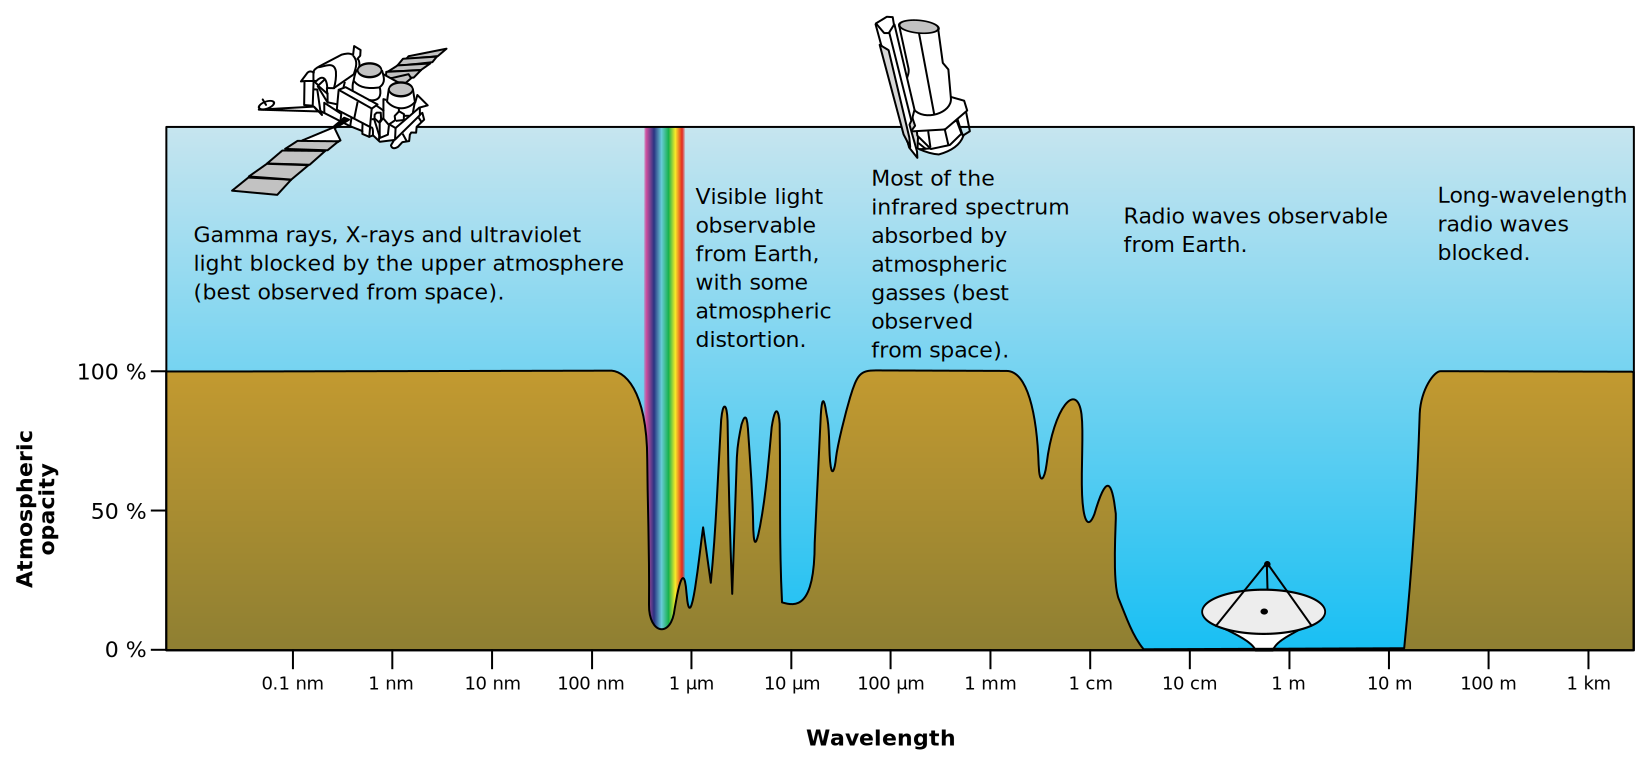
\includegraphics[width=\textwidth]{images/Atmospheric_electromagnetic_opacity}
\caption{Opacity of the Earth's atmosphere given different wavelength coming from space. Source \texttt{wikipedia}}
\label{fig:atmospheric-opacity}
\end{figure}

\begin{figure}[htbp]
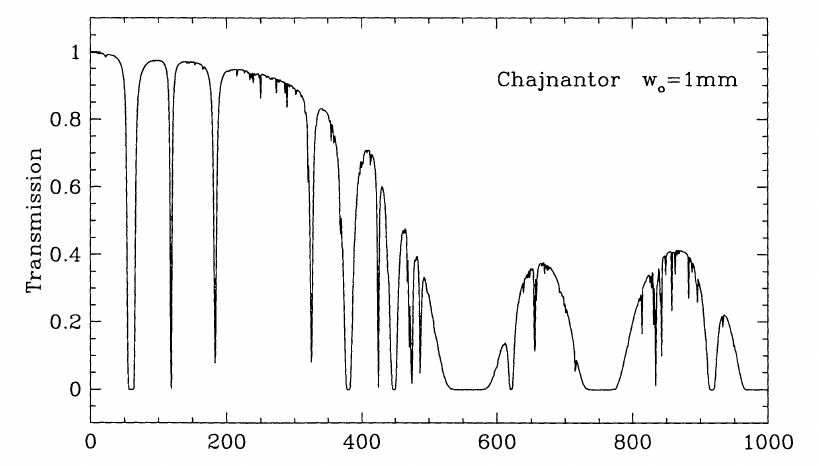
\includegraphics[width=\textwidth]{images/chajnantor-atm-transmission}
\caption{Transmission of the atmosphere from 0 to 1000 GHz for the ALMA site at Chajnantor in Chile assuming the typical value of $w_0 = 1 mm$ of precipitate water vapor. Source: \cite{taylor99}}
\label{fig:chaj-atm-tx}
\end{figure}

\begin{figure}[ht]
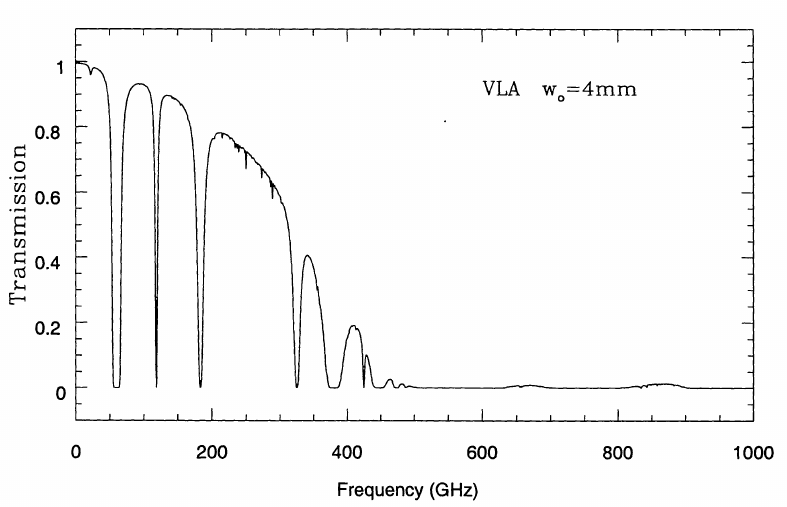
\includegraphics[width=\textwidth]{images/vla-atm-transmission}
\caption{Transmission of the atmosphere for VLA site in Socorro, NM, assuming a value of $w_0 = 4 mm$. Source: \cite{taylor99}}
\label{fig:vla-atm-tx}
\end{figure}

Figure \ref{fig:vla-atm-tx} shows the model of the atmospheric transmission at cm and mm wavelengths for the VLA site at 2150 m of altitude, figure \ref{fig:chaj-atm-tx} shows the model for ALMA site located in Chile at 4600 m of altitude. In both plots is possible to see a strong absorption lines including the water line at 22 GHz and 183 GHz, and the $O_2$ lines at 60 GHz and 118 GHz, plus a systematic decrease in the transmission with increasing frequency between lines. Every plot includes a different value for the column density of precipitable water vapor $w_0$ where each of one is typical for the site where the samples were taken. The precipitable water vapor (PWV) is the depth of the water vapor in the atmosphere in the site if it were converted to liquid phase.

(System temperature $T_{sys}$ is missing, explain definition and usage in the observation)

\subsection{ALMA Project Data Model}
\label{sec:apdm}
The ALMA Software system works using the concept of an Observing Project. The Observing Project is used throughout the ALMA software as the top level structure associated with a project resulting from a single observing proposal. In fact the Observing Project is a container for all the information relating to a project before it begins execution. During and following execution other data associated with the project are created and held in other structures, each of which holds a reference to the original observing project. Of particular interest is the Project Status structure, which holds a record of the execution status of the Project. The ALMA Project Data Model (APDM) defines the structure of both the Observing Project (ObsProject) and the execution status (ProjectStatus).

The Scheduling Block (SchedBlock or SB) is the atomic unit of observing for ALMA, any given science observation will usually be broken into many SBs, which may, or may not be executed in sequence. The ALMA Scheduling Software will decide on which SB to execute at any given time on the basis of which is the best to execute now. An SB as a canonical execution length of around 30 minutes, however in practice the SBs observation duration could be up to 2 hours, depending of the Observation program.

\subsubsection*{Observation Project Entity}
When a ALMA user submits a project to the Data Base, then the user is creating a ObsProject. Almost all the end-user tools in ALMA operates on ObsProjects, no other entities are exposed to the end user.

In order to hold all of the pre-observing information associated with a project the ObsProject entity class is composed of three parts: an ObsProposal, an ObsReview and an ObsProgram. These hold the information associated with the three phases of observing preparation: the proposal or Phase I, the reviewing and resultant approvals, and the observing program definition, or Phase II.

\subsubsection*{Observation Program Entity}
The Observing Program (ObsProgram) part of the Observing Project holds all the information created during Phase II, or program preparation. The ObsProgram consists of an Observing Plan (ObsPlan) and a SciencePlan. The Science Plan covers the science goal oriented view of the observing, and it is intended to contain the information that most users will use to define their observing programs. This information will persist, for the convenience of users, but will not be the definition that is used by the Observatory when carrying out the observations. Instead the latter information is contained within the ObsPlan, and covers what we call the system view. The service of Program Generation allows users to create the Observing Plan from their Science Plan. It is also possible for very advanced users to ignore the Science Plan and simply create all of the Observing Plan directly.

As stated, the Observing Plan (ObsPlan) is the container for defining the actual observing objects. In modeling terms the ObsPlan is a role for the top level ObsUnitSet, heading the definition of the system view. An ObsUnitSet contains a collection of Scheduling Blocks or more ObsUnitSets, along with objects defining the preconditions, performance and calibration requirements, and flow control that apply to that collection.

\subsubsection*{Scheduling Block Entity}
A Scheduling Block (SB) is the unit of observing for ALMA. It defines all the information that is required by the Observatory to independently execute the acquisition of a set of data and then to calibrate it as well. Since SBs are selected for execution individually they must exist as separate items in the data base.

Most of the structures within the SB hold information that is used either by the scheduler, to query whether or not this SB is suitable for scheduling ``now'', or as information that is used by the Observing Script (in the Control subsystem) to actually execute the observing (see below), and in some cases both. There are also performance goals for the SBs, to be measured against by the observing system.

So to allow the determination of ``Schedulability'' we find items like representative target observability, weather constraints, a precondition that requires a current Baseline Calibration and a Scientific Priority.

\subsubsection*{Targets}
The target is the element within an SB that defines the area to map, the spectral or instrumental setups to use, and the purpose of the observing. In fact the target element itself contains nothing except references to other elements that contain descriptions of these three key components.

\subsection{General problem}
\newtheorem{problem-def}{Definition}
The atomic unit to be scheduled is called scheduling block, this name matches the name described in section~\ref{sec:apdm}, although it differs since, the scheduling block defined as atomic unit here, considers only the representative target as the only considered target.
\begin{problem-def}
A Scheduling Block (SB) is represented as a n-tuple of time independent  properties ($P$). Let $S_0$ be the set of all SBs,
$$S_0 = P_1 \times P_2 \times ... \times P_n,$$
for appropriate $P_i$ sets. Then one SB is:
$$sb = (p_1, p_2, ..., p_n) \mid p_i \in P_i$$
\end{problem-def} 

Once defined a scheduling block, then the operation of selecting SB can be defined as:
\begin{problem-def}
The scheduling blocks selection is represented as a function that for a given time $t$ and a set of SBs $S \subseteq S_0$, it returns a subset of S:
$$sel:(t,S) \rightarrow \mathcal P \left({S}\right)$$
\end{problem-def}

Given these definitions, a property of $sel$ follow:

\newtheorem{sel-props}{Property}
\begin{sel-props}
The full selection operation $sel$ for a given time $t$ can be decomposed in independent selection operations, one for each property $p_i$:
$$sel(t,S) = sel_1(t, S) \cap sel_2(t, S) \cap ... \cap sel_n(t,S)$$
In general each one of these selection operations can be expressed  as an inequality:
$$sb \in sel_i(t, S)\,i.i.f\;\alpha_1(t, sb) \leq \alpha(t, sb) \leq \alpha_2(t, sb)$$
From now on this property will be called ``schedulable time window''.
\end{sel-props}

Without losing generality, the inequality of the property of above can be separated in two inequalities, then the condition can be expressed as: 
$$\alpha'(t, sb) \leq \alpha (t, sb)$$
Regarding the dependencies of both $\alpha$ and $\alpha'$, if the property depends on $t$, then the property is \textit{dynamic}, which means that the property is calculated and updated accordingly the scheduling algorithm progress. In other hand the properties depending only on $sb$ are \textit{dynamic} the values for them are pre-calculated at the beginning of the algorithm.\\

In general a sky source will be visible daily for hours then the source will go below horizon due the Earth's rotation, unless the source is circumpolar in which case the source will be always visible. Also the Earth's orbit movement around the sun would cause that a source will be visible during a period of the calendar year only. Both of these source properties are predictable and can be calculated. Nonetheless, the weather cannot be foreseen with exactitude, even the most accurate weather foresee could have a error margin which will increase if the period of time foresaw increase.

In common terms a Scheduling Block is ``schedulable'' only if the representative target for the given scheduling block is observable, this means that the source of the sky is visible, the array configuration has enough hardware capabilities to observe the source according to the scientific plan, the weather conditions are good enough to carry on the observation, etc. Basically this is the intersection of the different $sel$ functions and it is defined as the \textit{schedulable time window} for a given scheduling block, this window could be available several times during the observing season. In practical terms a scheduling block can be observed as many times as possible until it has been complete.

As stated in the section \ref{sec:apdm}, a scheduling block can have multiple targets, however the representative target is the most representative of the set of targets for the given scheduling block, which is selected by the creator of the Project/SchedBlock, thus this target will be the one used by the scheduler.

A scheduling block will be considered complete if it meets any of following three criterion:
\begin{itemize}
	\item \textit{Number of repetitions}: A scheduling block could have a limit of how many times can be observed.
	\item \textit{Total time observed}: A scheduling block could have a limit of how much time can be observed.
	\item \textit{Sensitivity achieved}: As stated in section \ref{sec:sens} if the goal for the RMS noise accumulated is achieved, then the scheduling block will be considered completed.
\end{itemize} 
Some of the scheduling blocks could not have all the three criteria, it is enough for the SB to have a least one of them.

The criteria to determine if a project was complete is based in how many scheduling blocks or ObsUnit sets have been completed or the total amount of time observed which is the sum of all the scheduling blocks observations. However, in reality human intervention is required to determine if the project has been completed based on the quality of science data extracted from the observations.

Every scheduling block execution is done in an \textit{Array} which is a subset of the available antennas in the observatory. Each antennas has its own hardware configuration to receive electromagnetic waves from the space. An array will have the hardware configuration common to all the antennas conforming the array, the idea is to observe the target with the same hardware in all the antennas as they were a single instrument. In general in an observatory all the antennas conforming an array will have all the same capabilities even they can be interchange each other and should not be any difference, however problems in some instruments during observatory operations could temporally remove some capabilities from some antennas.

Over the time available in the observing season is possible to have different \textit{Array configurations}. Each array configuration can be composed of 1 or more antennas available in the observatory, each one can offer different science capabilities which can be or cannot be used by the scheduling block, nevertheless each array will offer basic differences like the $uv$ coverage as seen in section \ref{sec:uvcover}, the angular resolution explained in section \ref{sec:angular-res} or the sensitivity achieved in every observation (section \ref{sec:sens}) which is dependent of the number of antennas in the array. As well one or more arrays can be available for observations at the same time, however each scheduling block must be observed by just one array at a given time.

Every project submitted to be observed in the observing season does not have the same science value, this means there are certain projects that are more interesting to observe and complete than others. This measure of how much value has a project is given by science team of the observatory, therefore the scheduler must be aware of this and try to complete most of the projects having the ``highest'' science qualification, this will be known as the \textit{scientific throughput}.

The \textit{scheduling array problem} consists on determine a schedule for the given set of scheduling blocks considering one or more arrays already created in a given period of time. The idea is to try to observe most of the projects with high scientific value in the less amount of time possible considering all the scientific requirements.


The \textit{array configuration schedule problem} is on top of the scheduling array problem. It consists in try to determine a schedule of observations for the observing season (which is a fixed amount of time and it lasts for several months, up to 1 year), for given set of the scheduling blocks and the given set the array configurations. The idea is to try to observe most of the projects with high scientific value considering all the scientific requirements during the observing season, however not all the projects could be completed.


\subsection{ALMA Scheduling Problem}
The Atacama Large Millimeter/submillimeter Array (ALMA) is a major collaboration effort between European, North American and East Asian countries, under construction on the Chilean Chajnantor plateau, at 5.000 meters altitude. When completed in 2013 it will be the largest radio telescope on earth, with more than 60 antennas of 12 and 7 meters diameter, distributed over a wide extension, with up to 16 kilo-meters of baseline separation. The ALMA interferometer will provide the possibility to be used as a single array, or as up to six (due to limited centralized equipment, photonic references) minor independent arrays or groups of antennas. As each array is equivalent to one instrument, this can eventually be seen as a multi-telescope problem. Also, the antennas will be changing their positions over the year, as different distributions will be used to exploit various kinds of observations. As ALMA does not observe in the visible spectrum, observations are not limited to night time only, thus a 24/7 operation with as small downtime as possible is expected. 

ALMA will operate exclusively in service mode. Therefore, the Scheduling software Subsystem is supposed to provide a fully automatic “quasi-real-time” dynamic scheduling platform, mostly with the only human participation of supervision. This Subsystem is still under development, and the needed algorithm(s) are still in a preliminary state. The main problem is the dynamic priorities scheduling, which differs widely from the traditional dynamic job-shop. This particular problem is very similar for all ground based observatories, and ALMA is one real example, that needs this kind of scheduling to accomplish its operations requirements.

The ALMA telescope will be operated as one or more antenna arrays, executing observation blocks corresponding to accepted project proposals. There will be three different antenna types, provided by three vendors:
\begin{itemize}
\item 12-m antennas (50): This is the main array to be operated, and also the one to be divided into several sub-arrays. They are provided by vendors Vertex (Vertex Antennatechnik GmbH) and AEM (Alcatel Alenia Space France, Alcatel Alenia Space Italy, European Industrial Engineering S.r.L., MT Aerospace).

\item 7-m antennas (12): This is the main part of the ALMA Compact Array (ACA), which will  operate as a separate array. They are provided by MElCo (Mitsubishi Electric Corporation).

\item 12-m total power antennas (4): These are special total power antennas able to see a full 2GHz spectrum, part of the ACA, but in principle exchangeable with any of the other 12-m antennas. They are also delivered by MElCo.

\end{itemize}

\begin{figure}	
\centering
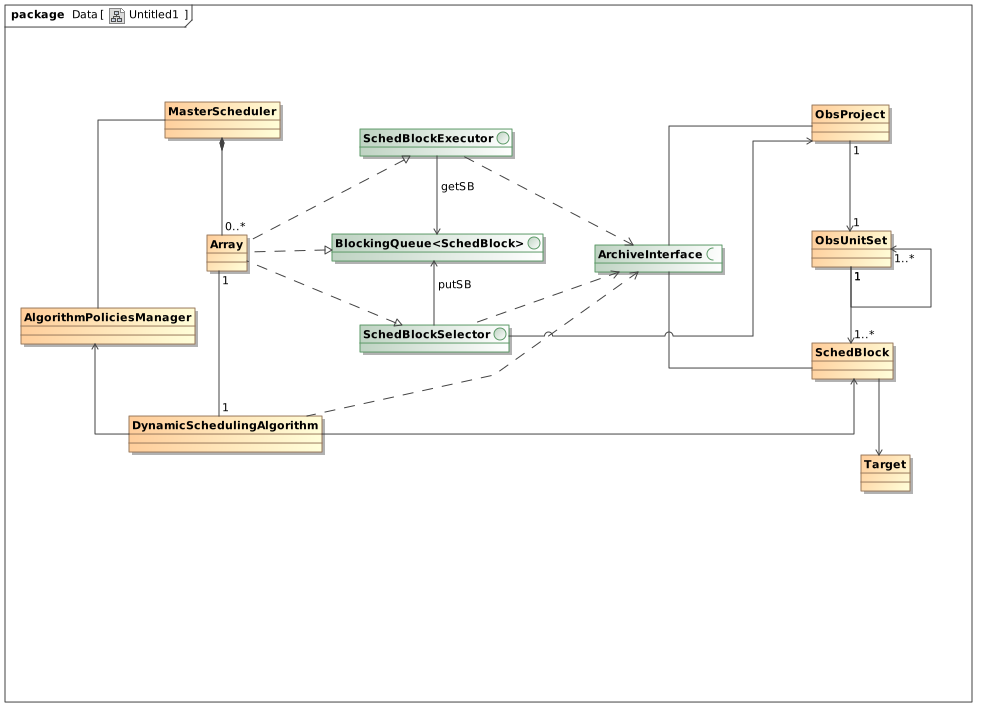
\includegraphics[width=\textwidth]{images/scheduling_class_model}
\caption{Basic class model of Scheduling subsystem. \texttt{MasterScheduler} and \texttt{Array} are the common classes used by all kind of Arrays. \texttt{DynamicSchedulingAlgorithm} is the class implemenenting the current ALMA's dynamic algorithm. At right side of the figure it is available the hierarchy of the the top level APDM classes used by the scheduling subsystem, which are accessed through the \texttt{ArchiveInterface}. } 
\label{fig:sched-class-model}
\end{figure}

A huge part of the telescope operations will be handled through the ALMA software, which is divided into various subsystems, such as Control, Correlator (ACA and Baseline), Pipeline, Archive, Scheduling and Offline software. The big picture of ALMA Software can be seen in \cite{schwarz04}.
The Scheduling Subsystem is the one in charge of managing antenna arrays and dynamically executing scheduling blocks. The current software design details are in \cite{clarke12}. The basic design considers 4 main parts which are represented in figure \ref{fig:sched-class-model}: The ``Master Scheduler'', The ``Array'', The ``Dynamic Scheduler instance'' and the ``Archive Interface''. The Master Scheduler is in charge of create and manage the creation of the Arrays and handle the management of the Scheduling Policies to be used in the DSA. The Array is the main operations unit of the scheduling subsystem, each array operates over Scheduling Blocks, executing, waiting for results of the observations and notifying to the user of the system what has been the outcome of the observation. The Array uses directly the Archive, which is the database storing the definition of each Observation project (see \ref{sec:apdm}), through the Archive Interface. Each array has its own scheduling queue, which can contain several schedblocks waiting to be executed, but just one SchedBlock is observed at the same time in each Array. Finally the DSA acts as a component of an Array selecting the current best SB according to the algorithm policy selected for the given Array, the details of the ALMA's DSA is discussed in section \ref{sec:alma-dsa}. Additionally each scheduling array can operate in 3 different modes: Manual, in this mode the scheduling queue is set with a maximum of one item, in this mode the user is responsible to execute the observation manually using low level scripts. Automatic, in this mode the array has a unlimited size scheduling queue, once a observation has been completed a new SchedBlock is taken from this queue to observe the next one until the queue is empty or the scheduler is stopped. And Dynamic, in dynamic mode the scheduling queue behaves as the array in interactive mode, but when the queue is empty the DSA is triggered selecting the next best SchedBlock to observe, depending if the DSA is active or passive the selected SchedBlock will be put in the queue to start the observation or the Scheduler will notify the user only respectively.

It is true that most of the scheduling software will be run in the online software, however there is a planning stage where the Scheduling algorithm will contribute to plan different scenarios of a season. The online usage of the algorithm is known as the \textit{short-term scheduler}, this scheduler can be used in quasi-real time or to planning the night observations. A \textit{medium-term scheduler} used to planning the observations of a frame of time where the array configurations are the same. And finally \textit{long-term scheduler} which should be able to plan an entire season of observation across the different planned array configurations, ideally the algorithm should define the duration of each configuration given as a input.  


\subsection{Comparison with classical scheduling problems}

The problem cannot be compared against job-shop due the scheduling block's schedulable time window, this does not allow to have every scheduling block available at any time. Besides this restriction, to observe at different times of the day the same target, ignoring weather conditions, would deliver different scientific result outputs due the nature of how the $uv$ coverage and sensitivity are calculated

To compare the astronomic scheduling problem against CPU scheduling also it could not be feasible. It is true that every SchedBlock is an atomic schedulable unit, like a process in a computer operating system, but when a schedblock is being observed it cannot be preempt to observe another schedblock, this limitations breaks most of the modern CPU scheduler designs found in modern operating systems. However it is possible to find some similitude with cooperative schedulers found in older operating systems. 

Another relaxation of this particular problem is the lack of obligation to complete all the projects for the given season. It is desirable to complete the projects with the highest scientific priority, however if one or more of the projects are not completed, they could re-appear in the next season because of the high scientific values assigned to them.


\begin{thebibliography}{9}
\bibitem{graham66}
	Graham R.,
	\textbf{Bounds for certain multiprocessing anomalies},
	Bell System Technical Journal,
	1966,
	45: 1563-1581.

\bibitem{hoogeveen04}
	Hoogeveen H,
	\textbf{Multicriteria scheduling},
	European journal of operational research,
	2004,
	167 (2005): 592-623.
	
\bibitem{thompson01}
	Thompson A. R, Moran J. M, Swenson Jr. G. W, 
	\textbf{Interferometry and Synthesis in Radio Astronomy},
	Wiley-VCH,
	2001,
	2nd edition,
	ISBN-13: 978-0471254928, ISBN-10: 0471254924.
	
\bibitem{taylor99}
	Taylor G. B, Carilli C. L, Perley R. A (eds.),
	\textbf{Synthesis Imaging in Radio Astronomy II},
	ASP Conference Series,
	1999,
	Vol 180.
	
\bibitem{gomez03}
	G\'omez de Castro A. I, Y\'a\~nez J,
	\textbf{Optimization of telescope scheduling Algorithmic research and scientific policy},
	 A\&A,
	 May III 2003,
	 Volume 403, Number 1: 357 - 367.
	 
\bibitem{mora11}
	Mora M.
	\textbf{A scheduling algorithm with dynamic priorities},
	Universidad T\'ecnica Federico Santa Mar\'ia, Departamento de Inform\'atica,
	2011.

\bibitem{johnston90}
	Johnston M. D,
	\textbf{Spike: AI scheduling for NASA's Hubble Space Telescope},
	Sixth Conference on Artificial Intelligence  Applications,
	May 1990,
	Vol 1, pages 184-190
	
\bibitem{zweben94}
	Zweben M, Fox M. S,
	\textbf{SPIKE: Intelligent Scheduling of HST Observations},
	Morgan Kaufmann Publishers,
	1994,
	Chapter 14, pages 391-422.

\bibitem{muscettola96}
	Muscettola N, Smith S. S,
	\textbf{Investigations into Generalizations of Constraint-Based Scheduling Theories with Applications to Space Telescope Observation Scheduling},
	Technical Report,
	The Robotics Inst., Carnegie-Mellon University,
	Pittsburgh, 1996

\bibitem{schwarz04}
	Schwarz J, Farris A, Sommer H,
	\textbf{The ALMA Software Architecture},
	SPIE,
	Proceedings of SPIE 2004, Advanced Software, Control and Communication system for astronomy.
	Volume 5496: 190-204

\bibitem{avarias11}
	Avarias J, Hiriart R.
	\textbf{ALMA Dynamic Scheduling Algorithm},
	NRAO Technical Report,
	2011.

\bibitem{clarke12}
	Clarke D, Lucero S, Farris A.
	\textbf{Scheduling subsystem design document},
	Technical Report,
	National Radio Astronomy Observatory,
	2012,
	COMP-70.55.00.00-003-F-DSN Version F

\bibitem{parekh93}
	Parekh, A. K, Gallager, R. G.
	\textbf{A Generalized Processor Sharing Approach to Flow Control in Integrated Services Networks: The Single Node Case},
	IEEE/ACM Transactions on Networking,	
	1(3):344-357,
	June 1993
	
\bibitem{li09}
	Li T, Baumberger D, Hahn S,
	\textbf{Efficient and scalable multiprocessor fair scheduling using distributed weighted round-robin},
	Proceedings of the 14th ACM SIGPLAN symposium on Principles and practice of parallel programming,
	1:65-74, ISBN: 978-1-60558-397-6
	4 April, 2009

\bibitem{chandra00}
 	Chandra A, Adler M, Goyal P, Shenoy P.
 	\textbf{fair scheduling: A proportional-share CPU scheduling algorithm for symmetric multiprocessor},
 	Proceedings of the 4th Symposium on operating System Design and Implementation,
 	pages 45-48,
 	October 2000
	
\end{thebibliography}

\end{document}
